\documentclass{report}
\usepackage{longtable}
\usepackage{listings}
\usepackage{graphicx}
\usepackage{multirow}
\usepackage{fontspec}
\usepackage[section]{placeins}

\newfontfamily{\ttconsolas}{Consolas}

\title{Lab5\_MUX/Decoder design}
\author{201704150 Kangjun Heo}

\lstset{basicstyle=\ttfamily,breaklines=true}
\lstset{framextopmargin=10pt,framexbottommargin=10pt,frame=tb}


\begin{document}
    \maketitle
    \tableofcontents

    \chapter{Purpose of the lab}

        \paragraph{This lab aims to design 4-to-1 Multiplexer and 2-to-4 Decoder with Verilog language. This report contains Truth table, Boolean equation, Karnaugh map and Logic diagram.}
    
        \section{Multiplexer}

        \subparagraph{\normalfont Multiplexer allows to pass desired amount of signals from multiple inputs. In this lab, the mulptiplexer takes 4 signals as input, and outputs 1 signal.}

        \section{Decoder}

        \subparagraph{\normalfont Decoder allows to express additional signals from lesser input. In this lab, the decoder takes 2 signals as input, and outputs 4 signals as outputs.}

    \chapter{Design Procedure}

        \section{Truth table and Karnaugh Map}
            \subsection{4-to-1 Multiplexer}

                \begin{longtable}{|l|l|l|l|l|l|l|l|l|l|l|l|l|l|}
                    \hline
                    A & B & C & D & E & F & Y & A & B & C & D & E & F & Y \\ \hline
                    0 & 0 & 0 & 0 & 0 & 0 & 0 & 1 & 0 & 0 & 0 & 0 & 0 & 0 \\ \hline
                    0 & 0 & 0 & 0 & 0 & 1 & 1 & 1 & 0 & 0 & 0 & 0 & 1 & 0 \\ \hline
                    0 & 0 & 0 & 0 & 1 & 0 & 0 & 1 & 0 & 0 & 0 & 1 & 0 & 0 \\ \hline
                    0 & 0 & 0 & 0 & 1 & 1 & 1 & 1 & 0 & 0 & 0 & 1 & 1 & 0 \\ \hline
                    0 & 0 & 0 & 1 & 0 & 0 & 0 & 1 & 0 & 0 & 1 & 0 & 0 & 1 \\ \hline
                    0 & 0 & 0 & 1 & 0 & 1 & 1 & 1 & 0 & 0 & 1 & 0 & 1 & 1 \\ \hline
                    0 & 0 & 0 & 1 & 1 & 0 & 0 & 1 & 0 & 0 & 1 & 1 & 0 & 1 \\ \hline
                    0 & 0 & 0 & 1 & 1 & 1 & 1 & 1 & 0 & 0 & 1 & 1 & 1 & 1 \\ \hline
                    0 & 0 & 1 & 0 & 0 & 0 & 0 & 1 & 0 & 1 & 0 & 0 & 0 & 0 \\ \hline
                    0 & 0 & 1 & 0 & 0 & 1 & 1 & 1 & 0 & 1 & 0 & 0 & 1 & 0 \\ \hline
                    0 & 0 & 1 & 0 & 1 & 0 & 0 & 1 & 0 & 1 & 0 & 1 & 0 & 0 \\ \hline
                    0 & 0 & 1 & 0 & 1 & 1 & 1 & 1 & 0 & 1 & 0 & 1 & 1 & 0 \\ \hline
                    0 & 0 & 1 & 1 & 0 & 0 & 0 & 1 & 0 & 1 & 1 & 0 & 0 & 1 \\ \hline
                    0 & 0 & 1 & 1 & 0 & 1 & 1 & 1 & 0 & 1 & 1 & 0 & 1 & 1 \\ \hline
                    0 & 0 & 1 & 1 & 1 & 0 & 0 & 1 & 0 & 1 & 1 & 1 & 0 & 1 \\ \hline
                    0 & 0 & 1 & 1 & 1 & 1 & 1 & 1 & 0 & 1 & 1 & 1 & 1 & 1 \\ \hline
                    0 & 1 & 0 & 0 & 0 & 0 & 0 & 1 & 1 & 0 & 0 & 0 & 0 & 0 \\ \hline
                    0 & 1 & 0 & 0 & 0 & 1 & 0 & 1 & 1 & 0 & 0 & 0 & 1 & 0 \\ \hline
                    0 & 1 & 0 & 0 & 1 & 0 & 1 & 1 & 1 & 0 & 0 & 1 & 0 & 0 \\ \hline
                    0 & 1 & 0 & 0 & 1 & 1 & 1 & 1 & 1 & 0 & 0 & 1 & 1 & 0 \\ \hline
                    0 & 1 & 0 & 1 & 0 & 0 & 0 & 1 & 1 & 0 & 1 & 0 & 0 & 0 \\ \hline
                    0 & 1 & 0 & 1 & 0 & 1 & 0 & 1 & 1 & 0 & 1 & 0 & 1 & 0 \\ \hline
                    0 & 1 & 0 & 1 & 1 & 0 & 1 & 1 & 1 & 0 & 1 & 1 & 0 & 0 \\ \hline
                    0 & 1 & 0 & 1 & 1 & 1 & 1 & 1 & 1 & 0 & 1 & 1 & 1 & 0 \\ \hline
                    0 & 1 & 1 & 0 & 0 & 0 & 0 & 1 & 1 & 1 & 0 & 0 & 0 & 1 \\ \hline
                    0 & 1 & 1 & 0 & 0 & 1 & 0 & 1 & 1 & 1 & 0 & 0 & 1 & 1 \\ \hline
                    0 & 1 & 1 & 0 & 1 & 0 & 1 & 1 & 1 & 1 & 0 & 1 & 0 & 1 \\ \hline
                    0 & 1 & 1 & 0 & 1 & 1 & 1 & 1 & 1 & 1 & 0 & 1 & 1 & 1 \\ \hline
                    0 & 1 & 1 & 1 & 0 & 0 & 0 & 1 & 1 & 1 & 1 & 0 & 0 & 1 \\ \hline
                    0 & 1 & 1 & 1 & 0 & 1 & 0 & 1 & 1 & 1 & 1 & 0 & 1 & 1 \\ \hline
                    0 & 1 & 1 & 1 & 1 & 0 & 1 & 1 & 1 & 1 & 1 & 1 & 0 & 1 \\ \hline
                    0 & 1 & 1 & 1 & 1 & 1 & 1 & 1 & 1 & 1 & 1 & 1 & 1 & 1 \\ \hline
                \end{longtable}

                \begin{table}[h]
                    \centering
                    \begin{tabular}{|c|l|c|c|c|c|c|c|c|c|}
                    \hline
                    \multicolumn{2}{|l|}{\multirow{2}{*}{}} & \multicolumn{8}{c|}{DEF}                                                                                                                                                                                              \\ \cline{3-10} 
                    \multicolumn{2}{|l|}{}                  & \multicolumn{1}{l|}{000} & \multicolumn{1}{l|}{001} & \multicolumn{1}{l|}{011} & \multicolumn{1}{l|}{010} & \multicolumn{1}{l|}{100} & \multicolumn{1}{l|}{101} & \multicolumn{1}{l|}{111} & \multicolumn{1}{l|}{110} \\ \hline
                    \multirow{8}{*}{ABC}        & 000       & 0                        & 1                        & 1                        & 0                        & 0                        & 1                        & 1                        & 0                        \\ \cline{2-10} 
                                                & 001       & 0                        & 1                        & 1                        & 0                        & 0                        & 1                        & 1                        & 0                        \\ \cline{2-10} 
                                                & 011       & 0                        & 0                        & 1                        & 1                        & 0                        & 0                        & 1                        & 1                        \\ \cline{2-10} 
                                                & 010       & 0                        & 0                        & 1                        & 1                        & 0                        & 0                        & 1                        & 1                        \\ \cline{2-10} 
                                                & 100       & 0                        & 0                        & 0                        & 0                        & 1                        & 1                        & 1                        & 1                        \\ \cline{2-10} 
                                                & 101       & 0                        & 0                        & 0                        & 0                        & 1                        & 1                        & 1                        & 1                        \\ \cline{2-10} 
                                                & 111       & 1                        & 1                        & 1                        & 1                        & 1                        & 1                        & 1                        & 1                        \\ \cline{2-10} 
                                                & 110       & 0                        & 0                        & 0                        & 0                        & 0                        & 0                        & 0                        & 0                        \\ \hline
                    \end{tabular}
                \end{table}


                \paragraph{$ Selection=\{A, B\}, Input=\{C, D, E, F\}, Output=Y $}
                \paragraph{BoolExp: $ Y = A'B'F + A'BE + AB'D + ABC $}
            
            \newpage
            \subsection{2-to-4 Decoder}
                \begin{table}[ht]
                    \centering
                    \begin{tabular}{|l|l|l|l|l|l|}
                    \hline
                    A & B & C & D & E & F \\ \hline
                    0 & 0 & 0 & 0 & 0 & 1 \\ \hline
                    0 & 1 & 0 & 0 & 1 & 0 \\ \hline
                    1 & 0 & 0 & 1 & 0 & 0 \\ \hline
                    1 & 1 & 1 & 0 & 0 & 0 \\ \hline
                    \end{tabular}
                \end{table}
                \begin{table}[ht]
                    \centering
                    \begin{tabular}{|c|c|c|c|c|c|c|c|c|c|}
                        \hline
                        \multicolumn{2}{|c|}{\multirow{2}{*}{}} & \multicolumn{2}{c|}{B} & \multicolumn{2}{c|}{B} & \multicolumn{2}{c|}{B} & \multicolumn{2}{c|}{B} \\ \cline{3-10} 
                        \multicolumn{2}{|c|}{}                  & 0          & 1         & 0          & 1         & 0          & 1         & 0          & 1         \\ \hline
                        \multirow{2}{*}{A}          & 0         & 0          & 0         & 0          & 0         & 0          & 1         & 1          & 0         \\ \cline{2-10} 
                                                    & 1         & 0          & 1         & 1          & 0         & 0          & 0         & 0          & 0         \\ \hline
                        \multicolumn{2}{|l|}{}                  & \multicolumn{2}{c|}{C} & \multicolumn{2}{c|}{D} & \multicolumn{2}{c|}{E} & \multicolumn{2}{c|}{F} \\ \hline
                    \end{tabular}
                \end{table}
                \paragraph{$ Input=\{A, B\}, Output=\{C, D, E, F\} $}
                \paragraph{BoolExp: $ C = AB $ $ D = AB' $ $ E = A'B $ $ F = A'B' $}
        \newpage
        \section{Logic Diagram}
            \begin{figure}[ht]
                \centering
                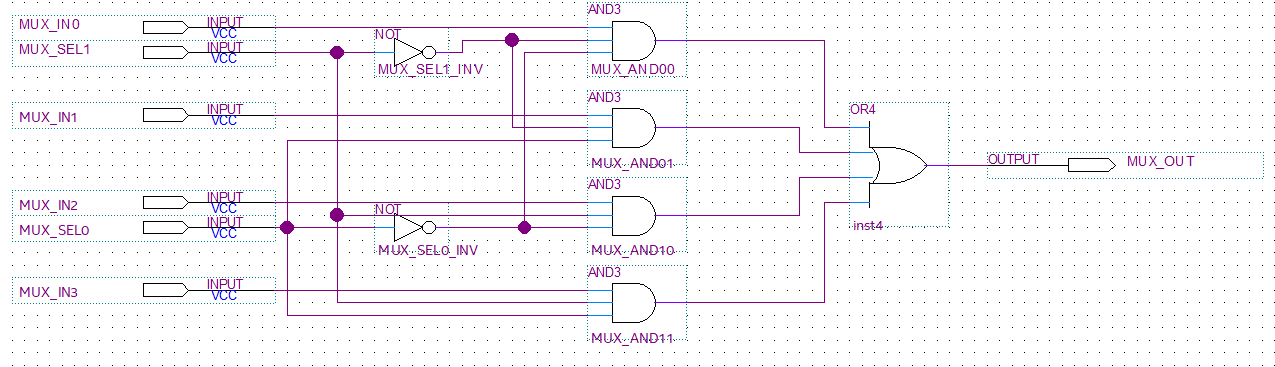
\includegraphics[width=\textwidth]{diagrams/logic_mux.png}
                \caption{Logic Diagram for 4-to-1 Multiplexer}
            \end{figure}
            \begin{figure}[ht]
                \centering
                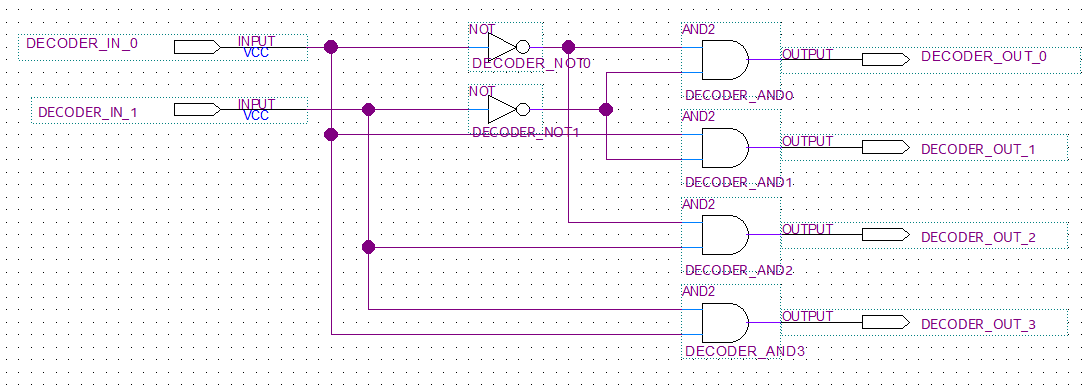
\includegraphics[width=\textwidth]{diagrams/logic_decoder.png}
                \caption{Logic Diagram for 2-to-4 Decoder}
            \end{figure}
    \chapter{Simulation}

        \section{Source Code}
            \subsection{Structural Style}

            \begin{figure}[ht]
                \centering
                \lstinputlisting{mux/st_4to1_mux.v}
                \caption{Structural Style Verilog Code of 4-to-1 MUX}
            \end{figure}

            \begin{figure}[ht]
                \centering
                \lstinputlisting{decoder/st_decoder_2to4.v}
                \caption{Structural Style Verilog Code of 2-to-4 Decoder}
            \end{figure}
            
            \subsection{Dataflow Style}

            \begin{figure}[ht]
                \centering
                \lstinputlisting{mux/df_4to1_mux.v}
                \caption{Dataflow Style Verilog Code of 4-to-1 MUX}
            \end{figure}

            \begin{figure}[ht]
                \centering
                \lstinputlisting{decoder/df_decoder_2to4.v}
                \caption{Dataflow Style Verilog Code of 2-to-4 Decoder}
            \end{figure}

            \newpage
            \subsection{Behavioral Style}

            \begin{figure}[ht]
                \centering
                \lstinputlisting{mux/bh_4to1_mux.v}
                \caption{Behavioral Style Verilog Code of 4-to-1 MUX}
            \end{figure}

            \begin{figure}[ht]
                \centering
                \lstinputlisting{decoder/bh_decoder_2to4.v}
                \caption{Behavioral Style Verilog Code of 2-to-4 Decoder}
            \end{figure}

        \section{Testbench} 
            \begin{figure}[ht]
                \centering
                \lstinputlisting{mux/tb_4to1_mux.v}
                \caption{Testbench Verilog Code of 4-to-1 MUX}
            \end{figure}
            \begin{figure}[ht]
                \centering
                \lstinputlisting{decoder/tb_decoder_2to4.v}
                \caption{Testbench Verilog Code of 2-to-4 Decoder}
            \end{figure} 

        \section{Simulation Result}
            \begin{figure}[ht]
                \centering
                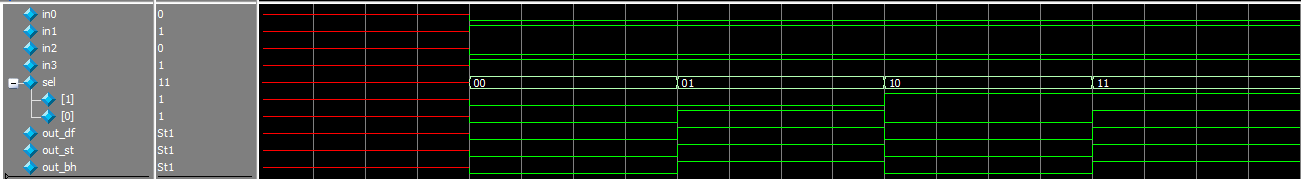
\includegraphics[width=\textwidth]{diagrams/waveform_mux.PNG}
                \caption{Waveform: 4-to-1 Multiplexer}
                \label{fig:waveform-mux}
            \end{figure} 
            
            \begin{figure}[ht]
                \centering
                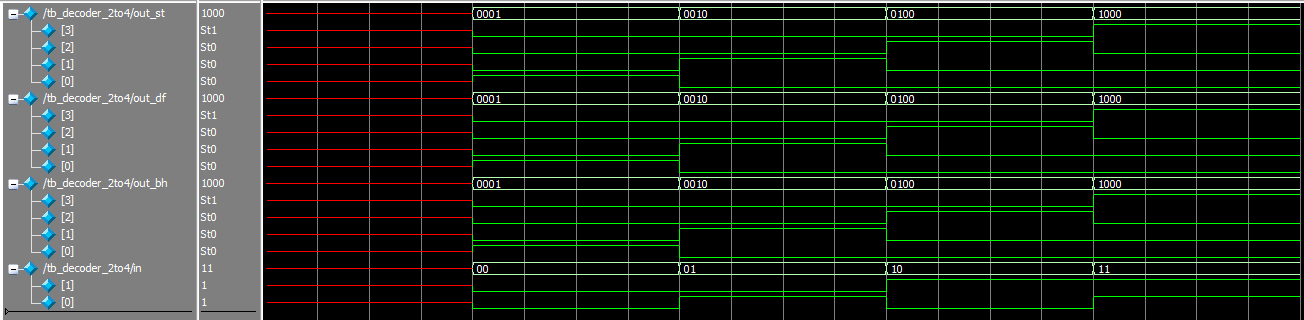
\includegraphics[width=\textwidth]{diagrams/waveform_decoder.PNG}
                \caption{Waveform: 2-to-4 Decoder}
                \label{fig:waveform-decoder}
            \end{figure} 
    \chapter{Evaluation}
        \paragraph{\normalfont First, The 4-to-1 Multiplexer gets input signal \texttt{0101}, and the selectional signal proceeds \texttt{00} to \texttt{11}. The output sequence should be \texttt{0101}. According to Figure ~\ref{fig:waveform-mux}, waveforms are generated as expected.}

        \paragraph{\normalfont The 2-to-4 Decoder gets input signal that proceeds \texttt{00} to \texttt{11}. The output sequence should be \texttt{0001}, \texttt{0010}, \texttt{0100}, \texttt{1000} for each progress. According to Figure ~\ref{fig:waveform-decoder}, waveforms are generated as expected. }

        \paragraph{\normalfont Therefore, the modules are properly designed.}
    \chapter{Discussions}
        \section{Key Part of This Lab}
        
        \paragraph{\normalfont Intel Quartus, The new development tool in this lecture makes assignments much harder because of its novelty caused several confusional mistakes. Also, Verilog is referred as "Similar as C", however, minor differences induced massive compilation error. So I needed to change my mind for it.}

        \paragraph{\normalfont Structural style description is intuitive, easily understand and translated as logic diagrams like as planned. But its source code can be boilerplate when the hardware becomes large. Dataflow style description helps developer's understadings how each datum flows. However, compiler creates complex RTL diagram. Behavioral style description literally defines "Behavior" or specific module. With \texttt{always} keyword developer defines how the module behave, so simple RTL diagrams will be created.}

        \section{Mistakes}

        \paragraph{\normalfont Unlike C, or any other C-like languages for Software Development, Verilog has bizarre syntax about ;(semicolon). Semicolons are similar with colon, it caused errors when I declare a module.}

        \section{Expected Improvements}

        \paragraph{\normalfont Designs are accomplished as in ideal form in gate level, however better testbench design is required. Its efficiency hardly reaches software testing's one, but part of the methodology can be applied.}
\end{document}